\hypertarget{ursula-buffay}{%
\section{Ursula Buffay}\label{ursula-buffay}}

\begin{figure}[!ht]
  \begin{adjustwidth}{-\oddsidemargin-1in}{-\rightmargin}
    \centering
    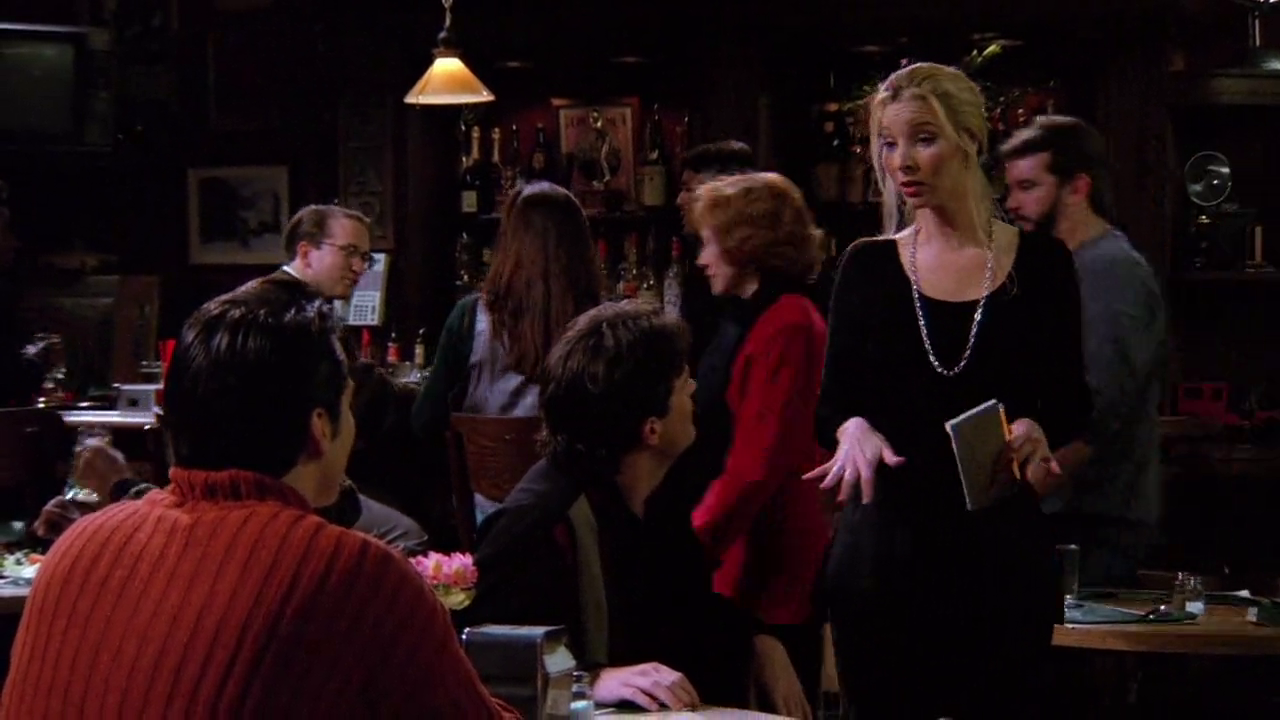
\includegraphics[trim={0 8cm 0 2cm,}, clip, width=\paperwidth]{./S01/img/16/ursula-buffay.png}
    % \caption{Ursula Buffay\label{fig:ursula-buffay}}
  \end{adjustwidth}
\end{figure}

Nesse episódio conhecemos Ursula, irmã gêmea da Phoebe. Ursula é,
originalmente, uma personagem da série \emph{Mad About You} (1992-1999).
Quando Lisa Kudrow foi chamada para o elenco de Friends os produtores
decidiram fazer um \emph{crossover} com a série, já que \emph{Mad About
You} também se passa em Nova Iorque.\footnote{\sloppy Ursula Buffay - Fandom Wiki. \url{https://friends.fandom.com/wiki/Ursula_Buffay}}

\hypertarget{liam-neeson-e-morley-safer}{%
\section{Liam Neeson e Morley Safer}\label{liam-neeson-e-morley-safer}}

\begin{figure}[!ht]
  \begin{adjustwidth}{-\oddsidemargin-1in}{-\rightmargin}
    \centering
    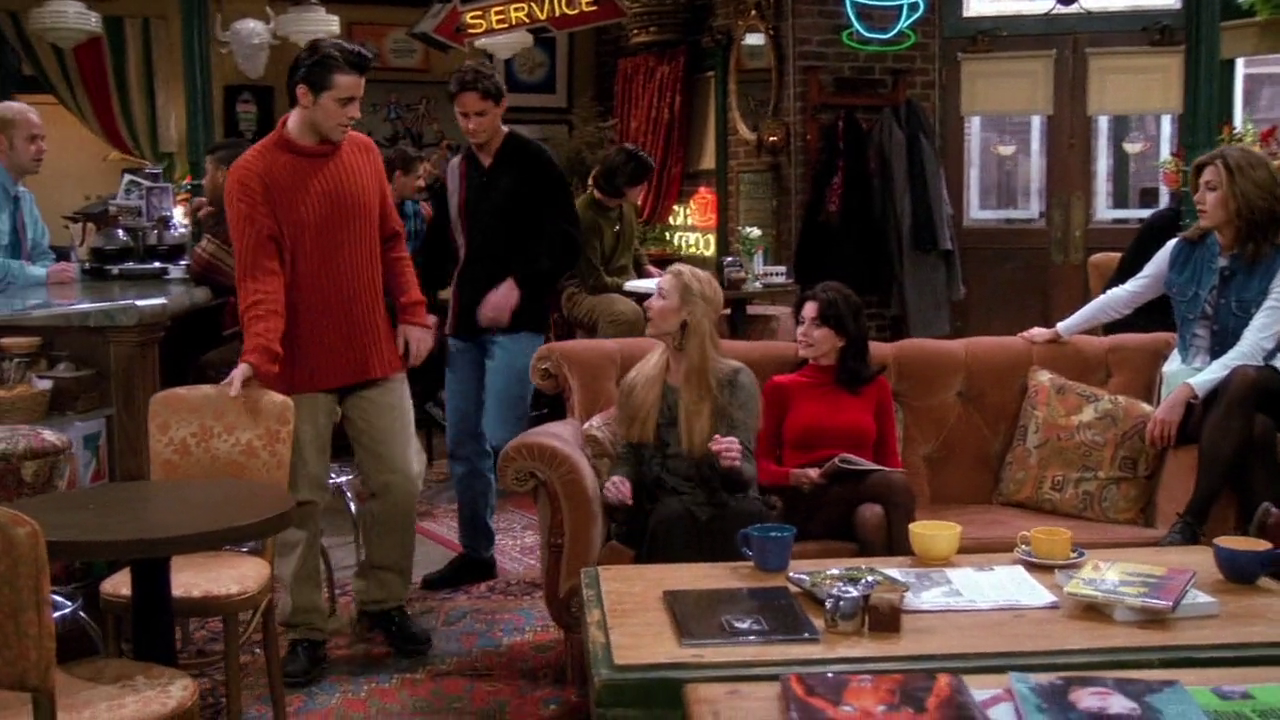
\includegraphics[trim={0 7cm 0 1cm,}, clip, width=\paperwidth]{./S01/img/16/liam-neeson-e-morley-safer.png}
    % \caption{Liam Neeson e Morley Safer\label{fig:liam-neeson-e-morley-safer}}
  \end{adjustwidth}
\end{figure}

\begin{tcolorbox}[enhanced,center upper,
    drop fuzzy shadow southeast, boxrule=0.3pt,
    lower separated=false, breakable,
    colframe=black!30!dialogoBorder,colback=white]
\begin{minipage}[c]{0.16\linewidth}
  \raisebox{\dimexpr-\height+\ht\strutbox\relax}{
    \centering 
\includegraphics[width=1.4cm]{./assets/img/joey.png}
  }
   & \centering \scriptsize{Joey}
\end{minipage}
\hfill
\begin{minipage}[c]{0.8\linewidth}
  \textbf{- Hey, Pheebs. Guess who we saw today.}\\
  - Ei, Pheebs. Adivinha quem vimos hoje.
\end{minipage}

\medskip
\begin{minipage}[c]{0.16\linewidth}
  \raisebox{\dimexpr-\height+\ht\strutbox\relax}{
    \centering 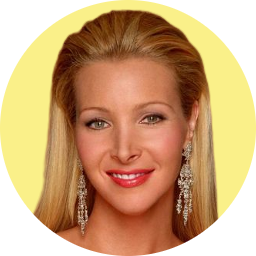
\includegraphics[width=1.4cm]{./assets/img/phoebe.png}
  }
   & \centering \scriptsize{Phoebe}
\end{minipage}
\hfill
\begin{minipage}[c]{0.8\linewidth}
  \textbf{- Liam Neeson. Morley Safer.}\\
  - Liam Neeson. Morley Safer.
\end{minipage}
\end{tcolorbox}

Joey tenta surpreender Phoebe com a notícia de que conheceu Ursula e faz
um jogo de adivinhação. Phoebe chuta \emph{Liam Neeson} (1952-) e
\emph{Morley Safer} (1931-2016).

\emph{Liam Neeson} é um ator norte-americano de ascendência irlandese
que, um ano antes de Friends estrear, faria um de seus papéis mais
emblemáticos no cinema interpretando \emph{Oskar Schindler} no filme
\emph{Schindler's List} (1993) ou \emph{A lista de Schindler} em
português, no qual \emph{Neeson} foi nomeado para o prêmio de melhor
ator no Oscar de 1994.\footnote{\sloppy Liam Neeson - Encyclopædia Britannica. \url{https://www.britannica.com/biography/Liam-Neeson}}

\emph{Morley Safer}, jornalista americano-canadense, se destacou na
cobertura da guerra do Vietnã e foi um dos correspondentes por 46 anos
do programa \emph{60 Minutes} da CBS.\footnote{\sloppy Morley Safer - Encyclopædia Britannica. \url{https://www.britannica.com/biography/Morley-Safer}}

No foto, \emph{Liam Neeson} à esquerda em seu papel de \emph{Oskar
Schindler}, e \emph{Morley Safer} à direita.

\begin{figure}
  \centering
  \begin{tikzpicture}
    \node [inner sep=0pt] at (0,0) {
      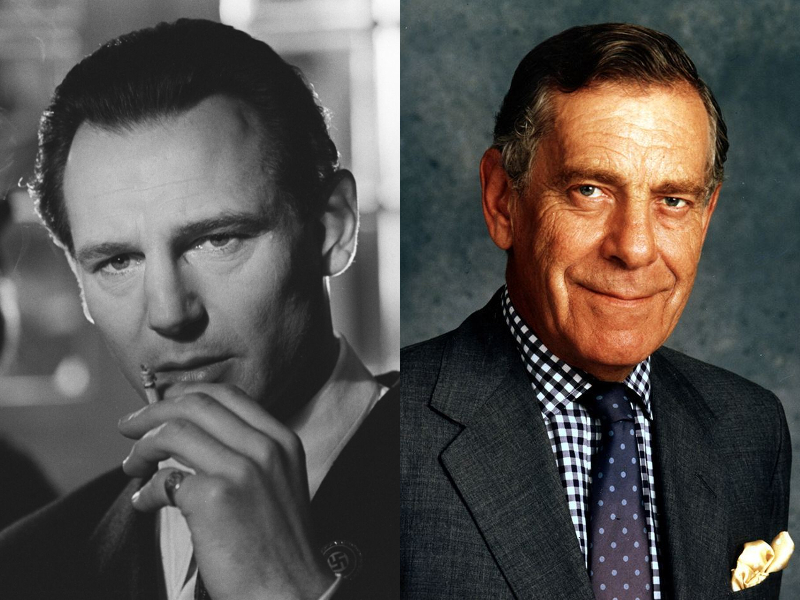
\includegraphics[width=0.8\textwidth,keepaspectratio]{./S01/img/16/liam-neeson-e-morley-safer-foto.png}
    };
    \draw [white, rounded corners=\ClipSep, line width=\ClipSep]
    (current bounding box.north west) --
    (current bounding box.north east) --
    (current bounding box.south east) --
    (current bounding box.south west) -- cycle
    ;
    \end{tikzpicture}
    \caption{Liam Neeson e Morley Safer\label{fig:liam-neeson-e-morley-safer}}
\end{figure}

\hypertarget{family-matters}{%
\section{Family Matters}\label{family-matters}}

\begin{figure}[!ht]
  \begin{adjustwidth}{-\oddsidemargin-1in}{-\rightmargin}
    \centering
    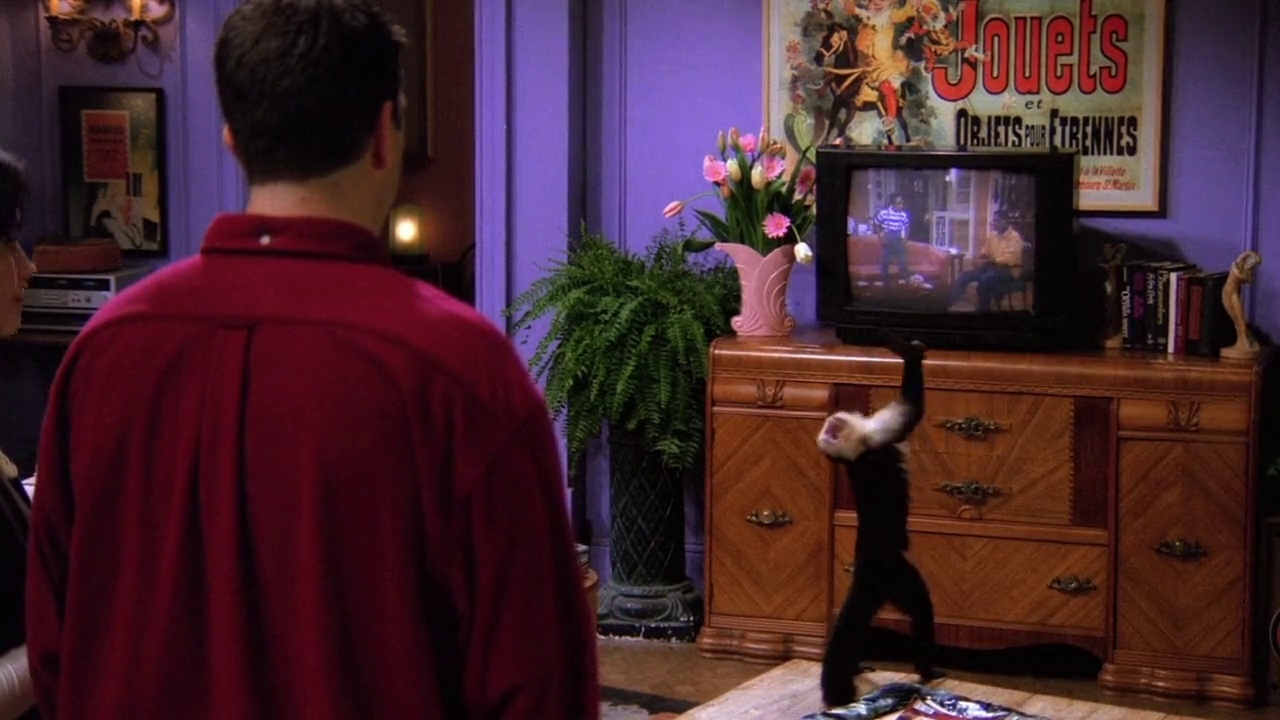
\includegraphics[trim={0 7cm 0 1cm,}, clip, width=\paperwidth]{./S01/img/16/family-matters.png}
    % \caption{Family Matters\label{fig:family-matters}}
  \end{adjustwidth}
\end{figure}

Com a TV ainda em modo SAP os amigos assistem a série \emph{Family
Matters} (1989-1998), \emph{sitcom} americana que conta a história de
uma família de classe média afro-americana que mora em
Chicago.\footnote{\sloppy Family Matters - Fandom Wiki. \url{https://familymatters.fandom.com/wiki/Family_Matters}}

\begin{tcolorbox}[enhanced,center upper,
    drop fuzzy shadow southeast, boxrule=0.3pt,
    lower separated=false, breakable,
    colframe=black!30!dialogoBorder,colback=white]
\begin{minipage}[c]{0.16\linewidth}
  \raisebox{\dimexpr-\height+\ht\strutbox\relax}{
    \centering 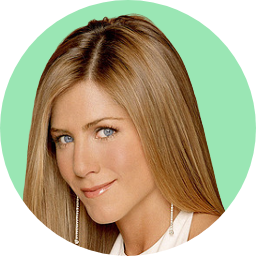
\includegraphics[width=1.4cm]{./assets/img/rachel.png}
  }
   & \centering \scriptsize{Rachel}
\end{minipage}
\hfill
\begin{minipage}[c]{0.8\linewidth}
  \textbf{- Oh, cool. Urkel in Spanish is Urkel.}\\
  - Que barato. Urkel, em espanhol, é Urkel.
\end{minipage}
\end{tcolorbox}

Rachel também menciona \emph{Urkel}, personagem que iniciou como
secundário na primeira temporada, mas logo se tornou um personagem
principal e um dos mais populares da série. Na foto, \emph{Urkel} é o
garoto de óculos e camisa amarela.\footnote{\sloppy Steve Urkel - Fandom Wiki. \url{https://familymatters.fandom.com/wiki/Steve_Urkel}}

\begin{figure}
  \centering
  \begin{tikzpicture}
    \node [inner sep=0pt] at (0,0) {
      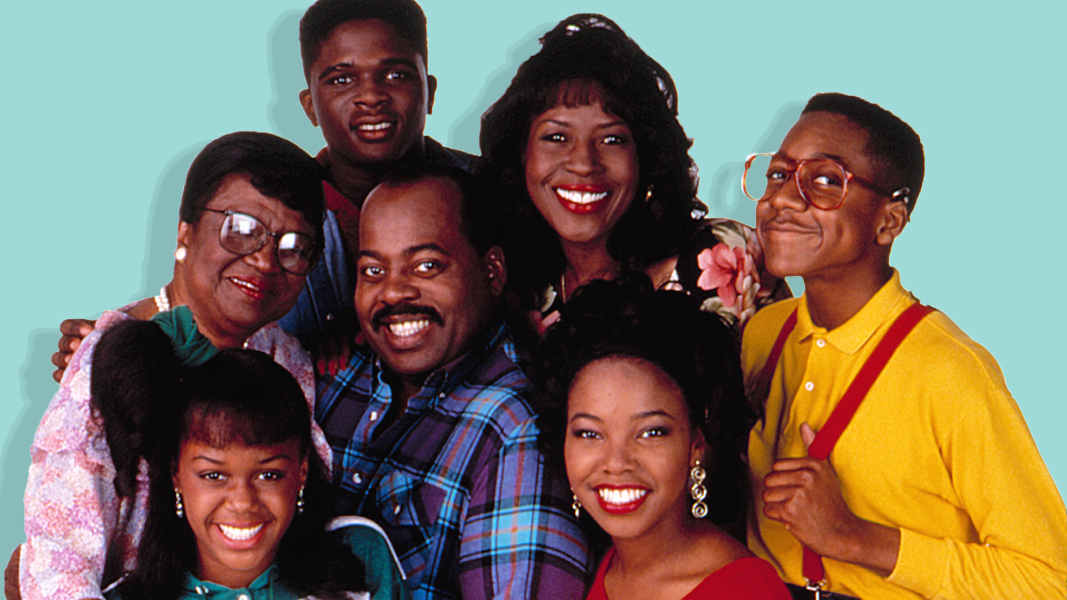
\includegraphics[width=0.8\textwidth,keepaspectratio]{./S01/img/16/family-matters-poster.jpg}
    };
    \draw [white, rounded corners=\ClipSep, line width=\ClipSep]
    (current bounding box.north west) --
    (current bounding box.north east) --
    (current bounding box.south east) --
    (current bounding box.south west) -- cycle
    ;
    \end{tikzpicture}
    \caption{Family Matters - Poster\label{fig:family-matters-poster}}
\end{figure}

\hypertarget{crabtree-evelyn}{%
\section{Crabtree \& Evelyn}\label{crabtree-evelyn}}

\begin{figure}[!ht]
  \begin{adjustwidth}{-\oddsidemargin-1in}{-\rightmargin}
    \centering
    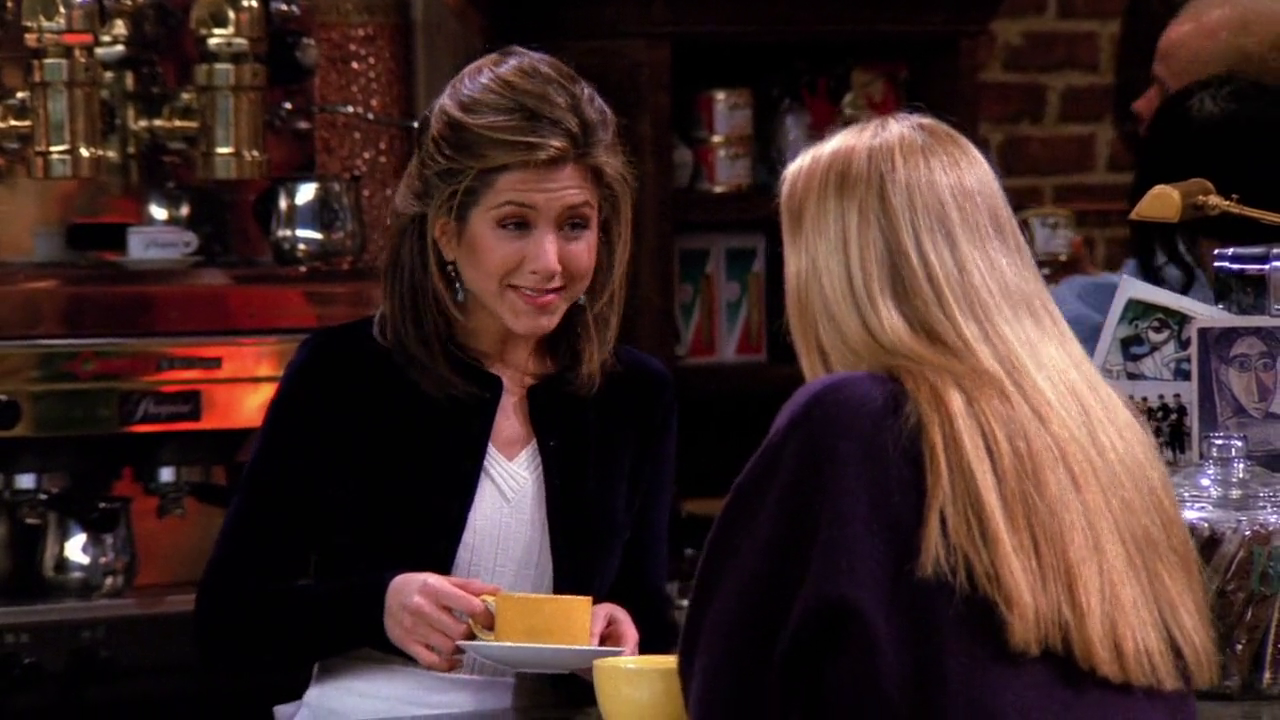
\includegraphics[trim={0 7cm 0 1cm,}, clip, width=\paperwidth]{./S01/img/16/crabtree-evelyn.png}
    % \caption{Crabtree & Evelyn\label{fig:crabtree-evelyn}}
  \end{adjustwidth}
\end{figure}

\begin{tcolorbox}[enhanced,center upper,
    drop fuzzy shadow southeast, boxrule=0.3pt,
    lower separated=false, breakable,
    colframe=black!30!dialogoBorder,colback=white]
\begin{minipage}[c]{0.16\linewidth}
  \raisebox{\dimexpr-\height+\ht\strutbox\relax}{
    \centering 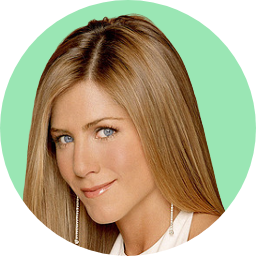
\includegraphics[width=1.4cm]{./assets/img/rachel.png}
  }
   & \centering \scriptsize{Rachel}
\end{minipage}
\hfill
\begin{minipage}[c]{0.8\linewidth}
  \textbf{- Anything from Crabtree \& Evelyn?}\\
  - Alguma coisa de Crabtree \& Evelyn?
\end{minipage}

\medskip
\begin{minipage}[c]{0.16\linewidth}
  \raisebox{\dimexpr-\height+\ht\strutbox\relax}{
    \centering 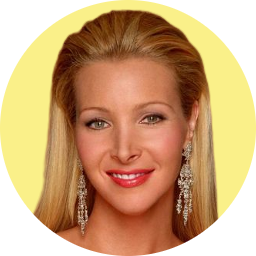
\includegraphics[width=1.4cm]{./assets/img/phoebe.png}
  }
   & \centering \scriptsize{Phoebe}
\end{minipage}
\hfill
\begin{minipage}[c]{0.8\linewidth}
  \textbf{- Bath salts would be nice.}\\
  - Sais de banho seriam uma boa.
\end{minipage}
\end{tcolorbox}

Rachel pergunta a Phoebe o que ela quer de aniversário. Quando Phoebe
menciona que o que ela realmente queria era que sua mãe estivesse viva e
comemorando com ela, Rachel pede algo mais simples e menciona
\emph{Crabtree \& Evelyn} (1971), loja varejista especializada em
produtos para higiene do corpo.\footnote{\sloppy Crabtree \& Evelyn - Site oficial. \url{https://www.crabtree-evelyn.com/pages/about-us}}

\hypertarget{jamie-e-fran}{%
\section{Jamie e Fran}\label{jamie-e-fran}}

\begin{figure}[!ht]
  \begin{adjustwidth}{-\oddsidemargin-1in}{-\rightmargin}
    \centering
    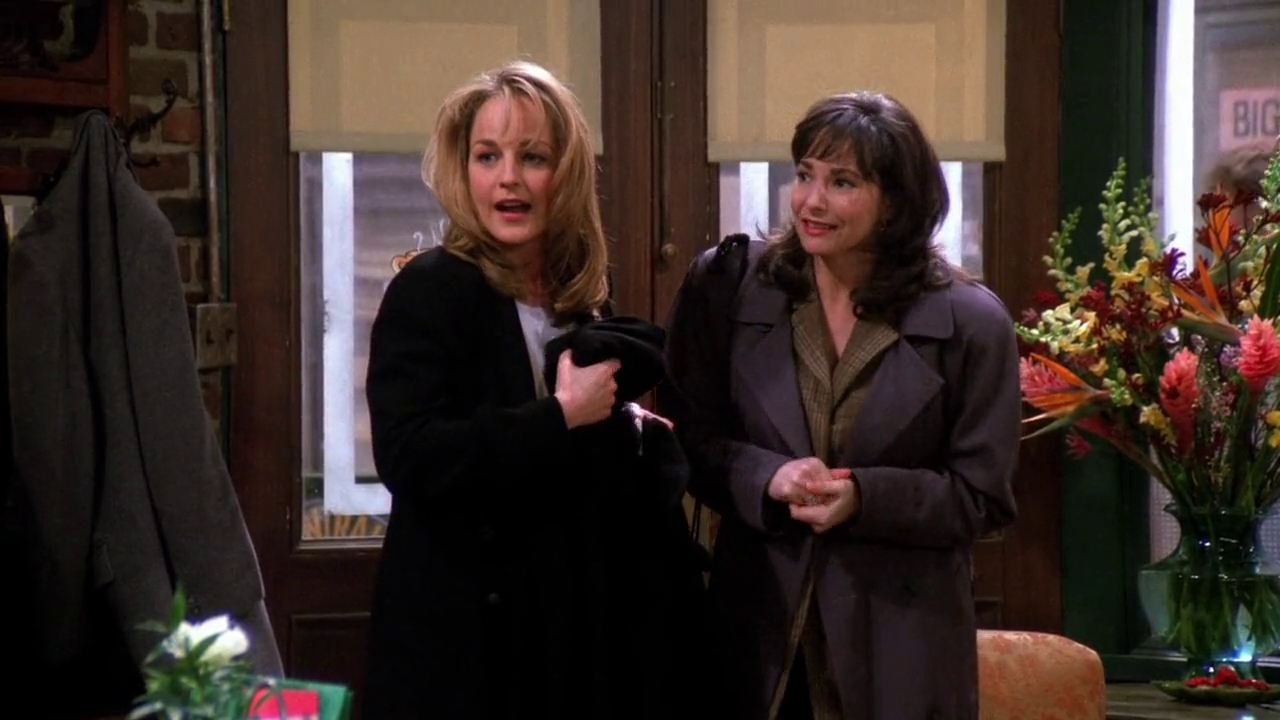
\includegraphics[trim={0 7cm 0 2cm,}, clip, width=\paperwidth]{./S01/img/16/jamie-e-fran.png}
    % \caption{Jamie e Fran\label{fig:jamie-e-fran}}
  \end{adjustwidth}
\end{figure}

Em mais um \emph{crossover} de \emph{Mad About You} vemos as personagens
\emph{Jamie} e \emph{Fran}, interpretadas por \emph{Helen Hunt}
(1963-)\footnote{\sloppy Helen Hunt - TMDB. \url{https://www.themoviedb.org/person/9994-helen-hunt}}
e \emph{Leila Kenzle} (1960-)\footnote{\sloppy Leila Kenzle - IMDB. \url{https://www.imdb.com/name/nm0005087/}},
respectivamente. Ne cena \emph{Jamie} e \emph{Fran} confundem Phoebe com
Ursula, e acham que ela foi demitida do \emph{Riff's}, restaurante que
também aparece em ambas as séries.

\hypertarget{laverne-shirley}{%
\section{Laverne \& Shirley}\label{laverne-shirley}}

\begin{figure}[!ht]
  \begin{adjustwidth}{-\oddsidemargin-1in}{-\rightmargin}
    \centering
    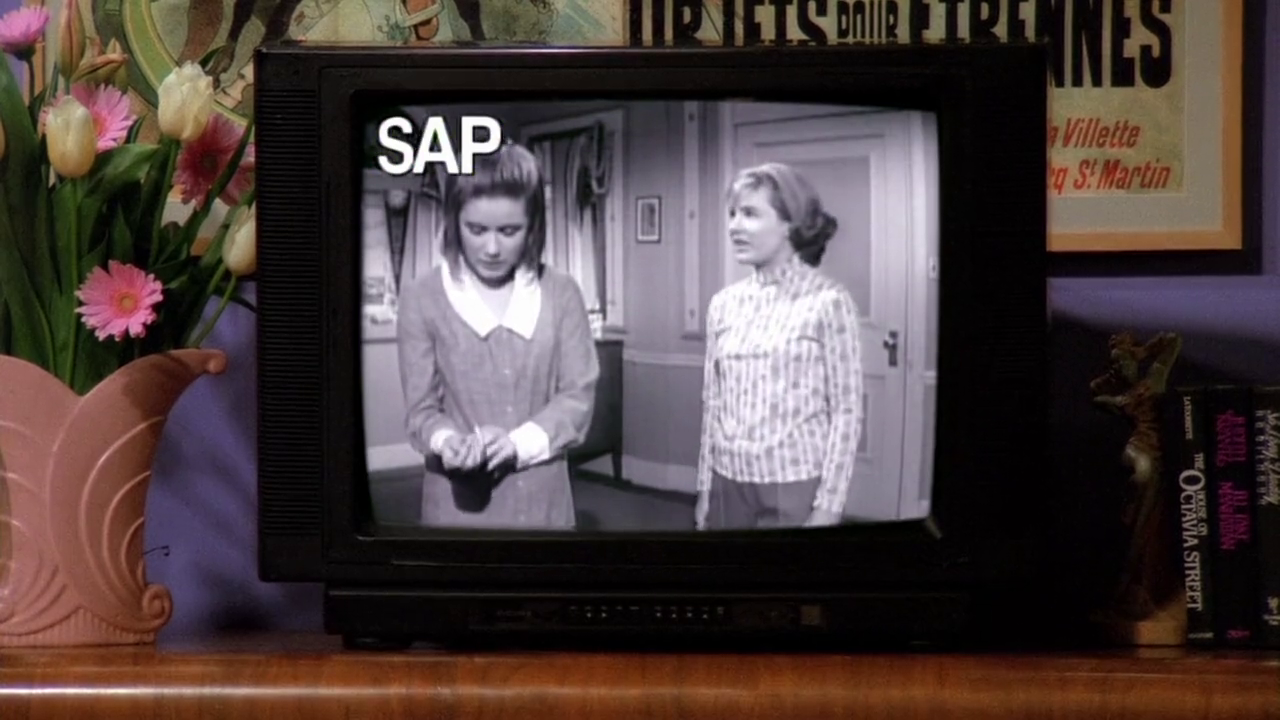
\includegraphics[trim={0 5cm 0 1cm,}, clip, width=\paperwidth]{./S01/img/16/laverne-shirley.png}
    % \caption{Laverne & Shirley\label{fig:laverne-shirley}}
  \end{adjustwidth}
\end{figure}

Os amigos assistem, ainda em espanhol, um episódio de \emph{Laverne \&
Shirley} (1976-1983), um \emph{spin-off} de \emph{Happy Days}. É uma
\emph{sitcom} americana que conta a história de \emph{Laverne DeFazio} e
\emph{Shirley Feeney} que trabalham em uma cervejaria em
Milwaukee.\footnote{\sloppy Laverne \& Shirley - Fandom Wiki. \url{https://bit.ly/3o9s1ol}}

\hypertarget{judy-jetson}{%
\section{Judy Jetson}\label{judy-jetson}}

\begin{figure}[!ht]
  \begin{adjustwidth}{-\oddsidemargin-1in}{-\rightmargin}
    \centering
    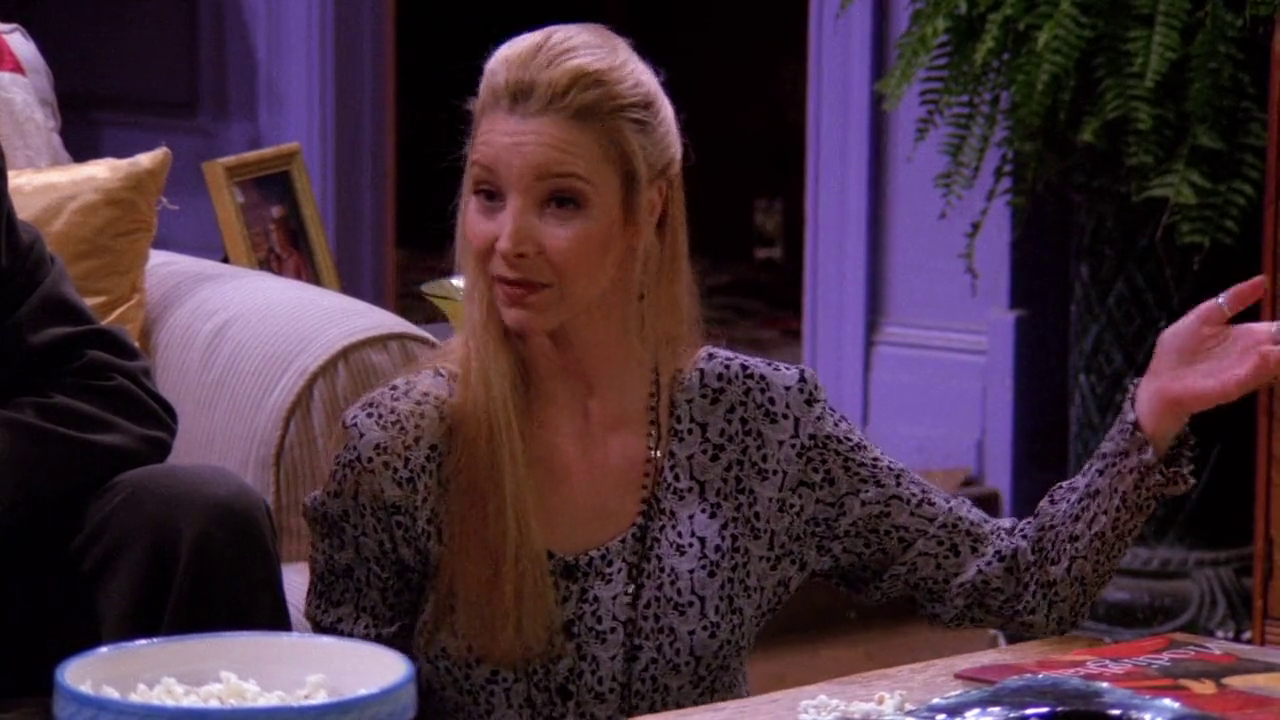
\includegraphics[trim={0 7cm 0 1cm,}, clip, width=\paperwidth]{./S01/img/16/judy-jetson.png}
    % \caption{Judy Jetson\label{fig:judy-jetson}}
  \end{adjustwidth}
\end{figure}

\begin{tcolorbox}[enhanced,center upper,
    drop fuzzy shadow southeast, boxrule=0.3pt,
    lower separated=false, breakable,
    colframe=black!30!dialogoBorder,colback=white]
\begin{minipage}[c]{0.16\linewidth}
  \raisebox{\dimexpr-\height+\ht\strutbox\relax}{
    \centering 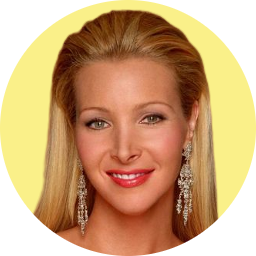
\includegraphics[width=1.4cm]{./assets/img/phoebe.png}
  }
   & \centering \scriptsize{Phoebe}
\end{minipage}
\hfill
\begin{minipage}[c]{0.8\linewidth}
  \textbf{- When I was 8, I wouldn't let her have my Judy Jetson Thermos, so she threw it under the bus.}\\
  - Aos oito anos, não deixei pegar minha garrafa térmica da Judy Jetson. Ela jogou embaixo do ônibus.
\end{minipage}
\end{tcolorbox}

Phoebe explica sua relação com a irmã na infância e menciona que Ursula
queria sua garrafa térmica da \emph{Judy Jetson}, personagem da série
animada \emph{The Jetsons} (1962-1987) produzida pela
\emph{Hanna-Barbera}, conhecida no Brasil como \emph{Os
Jetsons}.\footnote{\sloppy Judy Jetson - Fandom Wiki. \url{https://thejetsons.fandom.com/wiki/Judy_Jetson}}

Phoebe, num ato altruísta, presenteia Ursula com a garrafa térmica que
ela tanto queria quando criança no episódio seguinte,
\textbf{\textcolor{primarycolor}{S01E17 - Aquele com Duas Partes (Parte 2)}}.
Em troca Phoebe ganha o presente que Joey deu originalmente a Ursula, e
ela sabia disso mas nada disse.

\begin{figure}
  \centering
  \begin{tikzpicture}
    \node [inner sep=0pt] at (0,0) {
      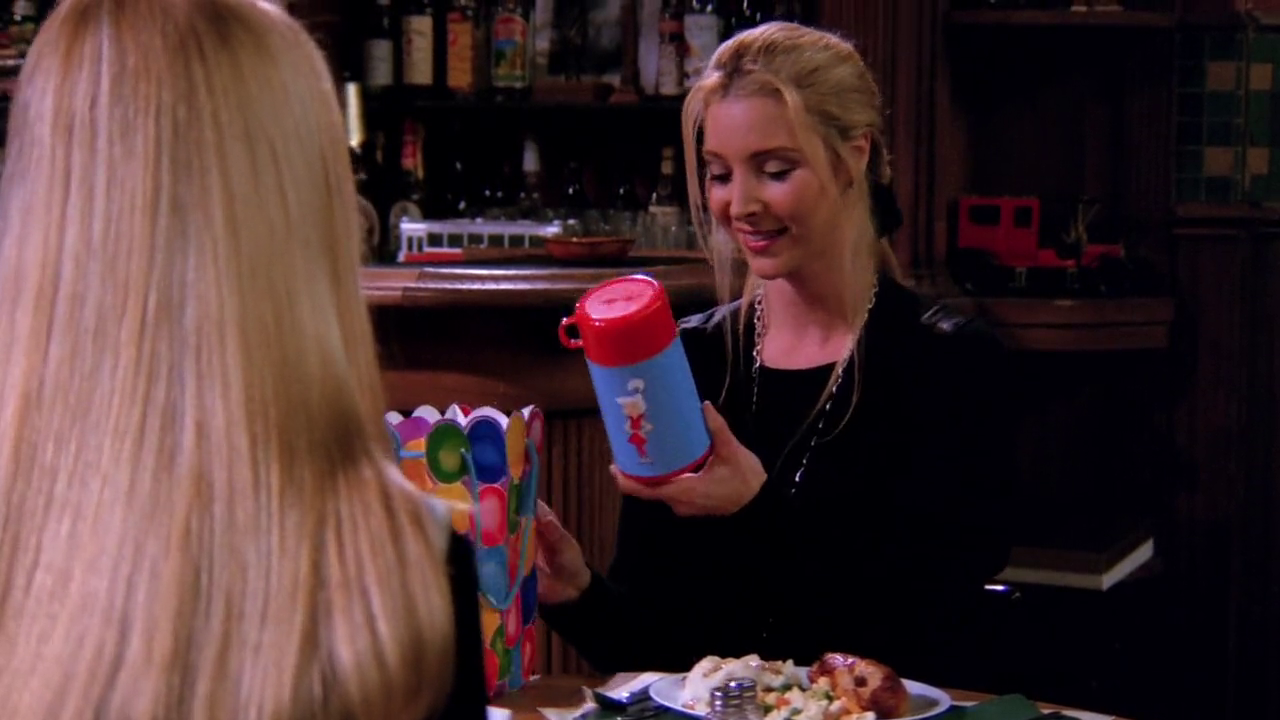
\includegraphics[width=0.8\textwidth,keepaspectratio]{./S01/img/16/garrafa-judy-jetson.png}
    };
    \draw [white, rounded corners=\ClipSep, line width=\ClipSep]
    (current bounding box.north west) --
    (current bounding box.north east) --
    (current bounding box.south east) --
    (current bounding box.south west) -- cycle
    ;
    \end{tikzpicture}
    \caption{Garrafa térmica da Judy Jetson\label{fig:garrafa-t-rmica-da-judy-jetson}}
\end{figure}
